

\newcommand{\Chip}[1]{\emph{\texttt{#1}}}
\newcommand{\MCX}[0]{\Chip{MC1322x}}
\newcommand{\RFA}[0]{\Chip{ATmega128RFA1}}
\newcommand{\Port}[1]{\emph{\texttt{Port #1}}}
\newcommand{\Comp}[1]{\emph{\texttt{#1}}}
\newcommand{\WPAN}[0]{\emph{LR-WPAN}}
\newcommand{\Tracker}[0]{\subsubsection{\emph{Tracked Issues}}\begin{description}}

\newcommand{\Contiki}[0]{\emph{Contiki}}
\newcommand{\ContikiOS}[0]{\emph{Contiki OS}}
\newcommand{\TinyOS}[0]{\emph{TinyOS}}


\documentclass[a4paper]{report}

\usepackage{multirow}
\usepackage{graphicx}

%% Comment out this for printing
\usepackage{hyperref}

\newcommand{\Href}[2]{\href{#1}{#2}} %% use this for proper href
%\newcommand{\Href}[2]{{#2}} %% fake version for printing

%% use \Href  and for printing we use \cite{something}
%% so we end up with link to the URL and bibliography
%% reference number as well. If \Href is fake there
%% will be no URL in the text.
\newcommand{\AltRef}[3]{\Href{#2}{#1} \cite{#3}}

\newcommand{\URL}[1]{\[ \href{#1}{\texttt{\emph{#1}}} \]}

%% Uncomment this for printing
%\usepackage{url} \newcommand{\URL}[1]{\[ \texttt{\emph{#1}} \]} \newcommand{\href}[2]{#2 (\texttt{\emph{\url{#1}}})}


\newcommand{\Issue}[1]{\Href{http://wmi.new-synth.info/issues/#1}{Issue \##1}}
\newcommand{\IssueX}[1]{\item[\Href{http://wmi.new-synth.info/issues/#1}{\Issue{#1}}]:}

\newcommand{\TEP}[1]{\AltRef{\emph{TEP#1}{http://www.tinyos.net/tinyos-2.x/doc/pdf/tep#1.pdf}{links:tinyos:tep:#1}}}

%% usage:
%	\MAN{gcc}
%	\MAN{2, open}

\newcommand{\MAN}[1]{\AltRef{\emph{\texttt{#1}{http://manpages.debian.net/cgi-bin/man.cgi\?query=#1\&sektion=0\&format=pdf}{\cite{doc:linux:man:0:#1}}}}}
\newcommand{\MANX}[2]{\AltRef{\emph{\texttt{#1}{http://manpages.debian.net/cgi-bin/man.cgi\?query=#2\&sektion=#1\&format=pdf}{\cite{doc:linux:man:#1:#2}}}}}


%% For this commands we need to use \Href explicitly
%% so if Href is proper - the display the path and link it
%% otherwise - just display the path. Because there's no
%% reason to show various refences to this in the bibtex

\newcommand{\Blob}[1]{\Href{https://github.com/errordeveloper/contiki-wmi/blob/wmi-work/#1}{\texttt{#1}}}
\newcommand{\Tree}[1]{\Href{https://github.com/errordeveloper/contiki-wmi/tree/wmi-work/#1}{\texttt{#1}}}
\newcommand{\Blame}[1]{\Href{https://github.com/errordeveloper/contiki-wmi/blame/wmi-work/#1}{\texttt{#1}}}

\usepackage{tikz}
\usetikzlibrary{automata,positioning,shapes,arrows}

\tikzstyle{C} = [diamond,
			draw, fill=blue!20,
			text width=4.5em, text badly centered,
			node distance=3cm, inner sep=0pt]

\tikzstyle{F} = [rectangle,
			draw, fill=green!20,
			text width=5em, text centered,
			rounded corners, minimum height=2.5em]

\tikzstyle{E} = [ellipse,
			draw, fill=red!20,
			node distance=3cm, minimum height=3em]

\tikzstyle{L} = [draw, -latex']

\usepackage{pstricks-add}

%\DeclareGraphicsExtensions{.eps,.epsi,.pdf,.png,.jpg}

\title{WMI: Wireless Music Instruments\\ \emph{BSc Final Year Project} \\ Final Report}
\author{Ilya Dmitrichenko \\ \\ Department of Computing\\ London Metropolitan University}

\date{\today}



\begin{document}
\maketitle


\abstract
{

   This an end of year report for BSc degree project which had originally targeted
  a design of complete wireless system for streaming of music control data collected
  from sensor devices and MIDI hardware to a host machine which would synthesise an
  audio signal the delivered into loudspeakers or recorded on disk. Despite rather
  simple design idea, the research and development had taken extended time period
  and the emphasis of this report is on a variety of aspects related to wireless
  network design and implementation. These aspects include cross-platform operating
  system architecture, microcontroller development hardware, application design and
  the abstraction layer requirements, hardware interfacing for the system and the
  application software as well as other miscellaneous subjects intersecting these
  areas. Two popular operating systems are presented in this report - \emph{Contiki}
  and \emph{TinyOS}. Two microcontroller architecture had been used in the course
  of this project - 32-bit \emph{ARM} and 8-bit \emph{AVR}. \emph{IEEE 802.15.4}
  devices where considered as the only suitable radio harware option, due to the
  wide use and availability of chips which implement this protocol. Another key
  assumption is that complice to the Internet Protocol (IP) is neccessary.

}

\tableofcontents
\listoffigures
%\listoftables

%%%%%%%%%%%%%%%%%%%%%%%%%%%%%%%%%%%%%%%%%%%%%%%%%%%%%%%%%%%%%%%%%%%%%%%%

\part{Introduction \& Research}
\part{Design \& Development} 
\chapter{Operating Systems for Wireless Sensor Networks}
\section{Overview of Embedded Operating Systems} \label{sec:RTOS}

		%% REWRITE !!

   A subject of extensive research for this project has been into the
  area of Real-Time Operating Systems for embedded devices, RTOS for short.
  This family of operating systems is not like any other general
  purpose OS family. The distinct feature that any RTOS has is the task
  management in constrained time-scale, the term \emph{real-time} is relatively
  abstract, it can be classified either as \emph{soft-} or \emph{hard-real-time}.
  The classification is also an abstract matter, some operating systems provide
  various approaches and it is up to the engineer to utilise it correctly for
  any given application. A modern RTOS should also provide a communication
  protocol stack and file storage drivers, support a set of platforms and
  a variety of peripheral devices.
 
 It is commonly known that RTOS is a rather expensive element in embedded design.
 This is because until very recently most commonly used RTOS implementations were
 provided only by specialised commercial vendors, brand names like \emph{Micrium},
 \emph{VxWorks} and perhaps \emph{QNX} are popular in specific application fields
 and there are also more obscure RTOS products offered at premium prices. Another
 more recent commercial RTOS is \emph{Nucleus}, currently owned by \emph{Mentor
 Graphics}. This repor does not focus on commercial products, hence these will
 not be refer to, more information can be found in \cite{wiki:rtos,wiki:rtos:list}.

 %http://en.wikipedia.org/wiki/Real-time_operating_system
 %http://en.wikipedia.org/wiki/List_of_real-time_operating_systems

 Currently the open sources community does present a number of very interesting
 RTOS projects, some of which are briefly introduced below. More details can be
 found on the WMI website \cite{wmi:wiki:rtos} (all the general project URLs are
 listed in that section of the website, and therefore omitted from the text below).
 It may be important to note that many of the project which are listed here are
 originating from major universities, some of which previously gave birth to very
 well know UNIX software and general innovations in the computer science.


 \subsubsection{RTEMS} \label{sec:rtos:rtems}

 The \emph{Real-Time Executive for Multiprocessor Systems} or \emph{RTEMS} is a
 full featured RTOS that supports a variety of open API and interface standards.
 It originates from US military and space exploration organisations. By definition
 \emph{RTEMS} is a highly scalable system, i.e. it is designed for multi-processor 
 deployment and is an interesting system to use for various possible applications,
 \emph{RTEMS} appears to be the oldest open-source RTOS. Unlike other systems below,
 the \emph{RTEMS} doesn't belong to sensor network OS sub-family on which this
 project had been focused. 


\subsubsection{TinyOS} \label{sec:rtos:tinyos}

 \emph{TinyOS} originates from the University of California, Berkeley and
 Stanford and the Intel Research Laboratory at Berkeley \cite{wiki:tinyos,
 links:tinyos:webs, links:tinyos:homepage}. The approach of \emph{TinyOS}
 is very different from all other systems, it uses a higher level abstraction
 language based on \emph{C}, which is called \emph{nesC}. It has a very
 modular semantics with degredd some similarity to hardware description
 languages (HDL), such as \emph{VHDL} or \emph{Verilog}. The name \emph{nesC}
 stands for "Network Embedded Systems C", in analogy with HDL it describes
 application level connectivity for modules, protocols and drivers. Despite
 this high level of abstraction, compiled source code is targeted for devices
 with limited compute resources \cite{links:tinyos:nesc}. The development
 ecosystem of \TinyOS\ also includes a network simulation package \emph{TOSSIM}
 \cite{links:tinyos:tossim}, which is a rather trivial element to design when
 such level of abstraction is in place. At the start of the project \TinyOS\
 was of some interest, however it had been opted out in preference to \Contiki\
 for it's more tradition \emph{"plain C"} language abstractions. However,
 \TinyOS\ had been evaluated during the development phase and more details
 can be found under section \ref{sec:TINYOS}.

 %http://en.wikipedia.org/wiki/TinyOS


\subsubsection{Nano-RK} \label{sec:rtos:nanork}

 \emph{Nano-RK} is a fully preemptive reservation-based RTOS, unlike
 any others in this section it already contained source code for \RFA\
 chip. The testing of \emph{Nano-RK} had been added to the project agenda.
 This OS is developed by Carnegie Mellon University and there are various
 interesting research papers available from the website
 \cite{links:nanork:pubs, pubs:nrk07, pubs:nrk06b, pubs:nrk06a, pubs:nrk06c}.
 Some particular features to mention are an implementation of real-time
 wireless communication protocol for voice signal transmission \cite{pubs:nrk06a}
 and a presence of an audio device driver within \emph{Nano-RK} kernel.

\TrackerList
	 \IssueX{21} Test Nano-RK on \RFA
\TrackerEnd



\subsubsection{Contiki - "The OS of Things"} \label{sec:rtos:contiki}

 {\emph{"Contiki is an open source, highly portable, multi-tasking operating
 system for memory-efficient networked embedded systems and wireless
 sensor networks. Contiki is designed for microcontrollers with small
 amounts of memory. A typical Contiki configuration is 2kB of RAM
 and 40kB of ROM.}}
 
 {\emph{"Contiki provides IP communication, both for IPv4 and IPv6. (\dots)}}
 
 {\emph{"Many key mechanisms and ideas from Contiki have been widely adopted in
 the industry. The uIP embedded IP stack, originally released in 2001, is today
 used by hundreds of companies in systems such as freighter ships, satellites
 and oil drilling equipment. (\dots) Contiki's protothreads, first released
 in 2005, have been used in many different embedded systems, ranging from
 digital TV decoders to wireless vibration sensors.}}
 
 {\emph{"Contiki introduced the idea of using IP communication in low-power
 sensor networks. This subsequently lead to an IETF standard and
 the IPSO Aliance (\dots)}}
 
 {\emph{"Contiki is developed by a group of developers from industry and
 academia lead by Adam Dunkels from the Swedish Institute of Computer
 Science."} \cite{contiki:home}

 Many publications by Adam Dunkels can be found on the SICS website
 \cite{dunkels04contiki, tsiftes09enabling}. He is also an author of
 two recent textbooks on IP WSN subject \cite{dunkels09operating,
 vasseur10interconnecting}. In addition, there is a rich set of simple
 code examples illustrating basic applications. The source code has
 well-defined directory hierarchy, build system and programming style
 \cite{contiki:code:style}.

 \emph{Contiki} provides a very simple API for advanced functions,
 such as real-time task scheduling, \emph{protothread} multitasking,
 filesystem access, event timers, TCP \emph{protosockets} and other
 networking features.

 More detailed description \emph{Contiki} is provided the following
 section (\ref{sec:CONTIKI}).
  

\section{Introducing the Contiki Operating System}\label{sec:CONTIKI}

  \Contiki\ operating system can be seen as collection of processes.
 In the same way as the UNIX operating system is seen as collection of
 files and processes. However, files are not a necessary component, in
 fact \emph{Coffee File System (CFS)} is only needed for some specific
 applications which require a non-volatile storage abstraction. 
  The inter-process communication (IPC) in UNIX has not been implement
 in the very early releases, although Contiki processes wouldn't work
 without its event-driven IPC mechanism\footnote{\emph{Though it is very
 primitive comparing to the usual meaning of IPC as an acronym.}}, which also
 drives the core scheduler. There is no notion of users in \Contiki\,
 however, and at this point comparison with UNIX becomes apparently
 impossible. Nevertheless, such a high-contrast comparison will hopefully
 deliver a good picture of what \ContikiOS\ is and what it is not.

% check the date in the slides from WSN course

  The lead developer of \Contiki\, Adam Dunkels of Swedish Institute of
 Computer Science (SICS), has revolutionised embedded system world by
 implementing \emph{lwIP} in 2000 and later, in 2002, even further optimised
 \emph{uIP} stack. It is known that until \emph{lwIP}, no complete IP stack
 existed which could run on a microcontroller device \cite{dunkels03full}.

  The key technique utilised in implementing \Contiki\ and the \emph{uIP}
 stack is based on a very obscure behaviour which the C language's
 \texttt{switch/case} statement exhibits in certain context. Dunkels
 wrote a few papers \cite{dunkels05protothreads,dunkels06protothreads}
 describing how it had been achieved, and summarises it in his doctoral
 thesis \cite{dunkels07programming}. The threading technique has been
 named \emph{protothreads (PT)}. Processes in \Contiki\ are designed as
 an extension to the \emph{protothreads}. Another extension is called
 the \emph{protosockets}, as the name suggest it provides the abstraction
 of network sockets.

  Most of functionality of all three key elements is delivered by the use
 of C pre-processor macros. The \emph{protothreads} are platform
 independent\footnote{\emph{It is not completely true for Contiki, there
 are few additions which utilise facilities that some hardware platforms provide.}}
 and can be integrated into any C program by including only one header file.
 \emph{Protothreads} can be used with virtually any C compiler and,
 as described in \cite{dunkels06protothreads}, the overhead is rather
 insignificant, considering the powerful functionality; the only limitation
 is due to the use of \emph{\texttt{switch/case}} statements by the \emph{PT}
 macros, these control structures will lead to undefined behaviour of the
 code in the \emph{PT} context.

  \emph{Protosockets} are designed specifically for \emph{uIP} and therefore 
 cannot be included with just one header. The only limitation of the
 \emph{protosockets} is due to design decision, there is no UDP communication
 facility, only TCP is provided. The \emph{protosockets} greatly simplify the
 application code, since all necessary functions are provided, including
 handling of strings. Thought no packet flushing is currently possible, which
 may be desired in some application.

\subsection{Initial Development Phase}

  \Contiki\ source code includes a large set of stable drivers for various
 RCBs which were mentioned previously, such as \emph{Zolertia Z1}, \emph{Tmote
 Sky}, \emph{Atmel Raven} and \Chip{RF230}\emph{-based} boards, \emph{TI}
 \Chip{CC2430} and \emph{MSP430} as well as \emph{ARM Conrtex-MX} and many
 older devices, including \emph{Comondore 64} and \emph{Apple II} computers.

 Details regarding the \Chip{MC1322x} port \cite{links:contiki:port:mc1322x}
 are to follow in \ref{sec:APPDEV}, since \Chip{MC1322x} was chosen as the
 target platfrom for this project. However, the \RFA\ platform had been the
 first preference. Major work during the inital phase had been done to
 port the existing driver code for \Chip{RF230} transceiver to take the
 advantage of the single chip device. This work had been described in the
 interim report \cite{wmi:irep}.


  A considerably long period of work during the first semester had been
 towards porting of \ContikiOS\ to run on \RFA\ chip. The details were
 included in the interim report \cite{docs:irep}. However, if the porting
 was to be completed, the time it would have taken may have exceeded the
 allocated period for the project (one academic year). Therefore it was
 uderstood that some reconsideration needed to be taken and two major
 solutions were proposed: either changing the development hardware or
 trying a different OS with the same hardware.

\subsubsection{Problems Ecountered while Proting the Driver Code}

  It had been not a trivial task to compare a set of implementations
 of the driver code, nevertheless some common fragments of code had
 been identified. The interinm report has included the details of what
 was acheived at the time, though most of work in this area \dots

\section{Outlook Trial for the TinyOS} \label{sec:TINYOS}

  It has been discovered that a few members of \TinyOS\ community
 have recently worked on porting \TinyOS\ to run on \Chip{ATmega128RFA1}
 \cite{tinyos:arch:rfa1-p1,tinyos:arch:rfa1-p2}. Comparing to \Contiki,
 \TinyOS\ has rather superior abstraction layer that provides a seamless
 cross-platform integration \cite{tinyos:tepXXX,tinyos:tepYYY,tinyos:tepZZZ}.
 
  Various internals of \TinyOS\ had been studied, however it is 
 certainly a very broad area to be described here. It is best described
 in the \emph{"TinyOS Programming"} book by David Gay and Philip Levis
 (it is available in print as well as a web-edition \cite{tinyos:book}).
 Two authors of this book are lead developer of the \TinyOS\ project
 and are currently working at the University of California, Berkley
 and Standford.


  \TinyOS\ currently had been ported to a variety of 8-, 16- and
 32-bit microcontrollers, most of the peripherals (such as I2C and SPI)
 have unified high-level access mechanisms, unlike in \Contiki\footnote{
 \emph{Most of peripheral drivers in Contiki OS are rather specific to
 a certain platform and only some particular drives share a similar
 interface.}}. Most of development documentation is provided in the
 the format of \emph{"TinyOS Enhancement Proposal"} (known as
 \emph{TEP}\footnote{\emph{These documents are commonly referred to as
 TEP\texttt{n}, where \texttt{n} is a number. \TEP{1} defines the format
 of the TEP documents.}}), there is also documentation generated from
 the source code comments (\emph{nescdoc}) as well as various on-line
 resources \cite{tos:wiki:docs} and the textbook mentioned above.
 It is noticeable that \TinyOS\ documentation is more extensive the
 what is currently presented for the \ContikiOS.


\subsection{Programming TinyOS: Compilers and Abstractions}

  The greatest achievement of \emph{TinyOS} is its specialised language,
 benefits of which had been overlooked at the earlier stage of research
 for this project. \emph{"Network Embedded Systems C" (nesC)} is a
 C-based language, it provides abstractions for components, interfaces
 and configurations. It is not an object-oriented language, though
 it is rather component and interface oriented. As it was defined in
 the previous section that \Contiki\ can be seen as a collection of
 processes and events are communicated between those processes, then
 \TinyOS\ can be defined as a collection of components and interfaces
 which are wired together in configuration abstraction layer, tasks,
 events and the data are communicated between the components via the
 interfaces.

  The control structures and all of C constructs are still valid in
 \emph{nesC}. This can be seen as if \emph{nesC}-specific statements
 are replaced by appropriate C source code that defines required behaviour.
 Nevertheless, this is only a brief description of the relation between
 \emph{nesC} and its ancestor. Just as if C could be defined by stating
 a ratio of lines of code in C versus lines of assembly code.

 It is important to note that current implementation of the compiler
 translates higher-level nesC code into C language. The resulting
 programs are specifically suited for embedded devices. Direct
 compilation would be possible and, if desired, there is an interesting
 platform to look into. \emph{LLVM} ("Low-level Virtual Machine") is a
 new generation compiler technology. It is know that using \emph{LLVM}
 and its family member \emph{clang} implementation of a new compiler
 for a C-like language would be simplified (comparing to more traditional
 techniques). One good example of industrial grade compiler based on
 \emph{LLVM} is the \emph{XC} toolchain for \emph{XS-1} devices from
 a UK semiconductor company \emph{XMOS} \cite{paper:xmos:docs:xcc}.

 Nevertheless, currently \emph{nesC} compiler is known to be fully
 functional and it's task is not as complex as it may seem. Programming
 in any language is always done by applying code patterns, general
 to some degree, to accomplish desired behaviour of a program.
 The purpose of \emph{nesC} abstraction layer can be seen as making
 the details of complex coding - with which high degree of modularity
 can be achieved - rather hidden away from the programmer.


\subsection{Network Protocols in TinyOS}
 
  \TinyOS\ has become widely adopted and there are many researchers
 who contributed significant work in different application areas, one
 such area of great interest to WMI project is sensor node timer
 synchronisation protocols. A number of papers are available and the
 mainstream repository of \emph{TinyOS} source code already contains
 implementations for some of those protocols.
 \emph{( A few details with references needed )}
  Further study and experimentation in this area are required to design
 a system which could cope with real-time constraints of stage control
 applications. It is important to note that \emph{P802.15.4} has addressed
 some real-time application requirements, however the status of software
 support for these features of \emph{P802.15.4} is currently uncertain.
 \emph{( Perhaps mention NanoRX ? )}

  After several aspects of \emph{TinyOS} were studied, it was clear
 that its current implementation of \emph{6loWPAN} is fully compatible
 with \emph{Contiki} and it had been desired to prove this in practice,
 but this has not been achieved at the time of writing of this paper.
  
  A problem exists however, there was no fully working IP-enabled driver
 for \emph{ATmega128RFA1} transceiver. The IP layers are provided by
 \emph{BLIP} stack (this stands for Berkley Lightweight IP), the stack
 is currently undergoing major development. Details on what is required
 are available on \emph{TinyOS} wiki page \cite{tinyos:wiki:blip-2-0},
 implementing it in \emph{nesC} was not as trivial due to the learning
 curve. Therefore this task had be postponed.

  This problem requires further explanation. \emph{TinyOS} has been
 developed since 2001, while \emph{Contiki} first dates back to two
 years later - 2003\footnote{\emph{No exact information has been
 found, these are the earliest dates which appear in the source code.}}. 
 In the early days of WSN research \emph{P802.15.4} and \emph{ZigBee}
 where still emerging, the \emph{6loWPAN} RFCs appeared at IETF more
 recently\footnote{\emph{The first revision of P802.15.4 was released
 in 2003 (current revision is from 2006) and first draft of 6loWPAN
 is dated April 2007.}}. \emph{TinyOS} has originally used its own
 protocol called \emph{ActiveMessage}.

  Currently \TinyOS\ incorporates \emph{BLIP} stack, which initially
 was released by UC Berkley Wireless Embedded Systems research group
 in the summer 2008, know as \emph{bl6lowpan} at that time \cite{ucb:webs:blip}.
 As mentioned below, major code changes are currently still in progress.
 The driver code which fully implements all new features of the \emph{BLIP}
 stack (including point-to-point tunnelling for simple UART wired
 connectivity) is only for the most popular \Chip{CC2420} radio chips.

\subsection{Hardware Resources}

  It is difficult to compare the two sets of what hardware platforms
 \TinyOS\ and \Contiki\ had been ported to, since the status of support
 for some platforms is uncertain. It is probably most appropriate to
 say that these two sets are almost equal, however, some platforms
 which appear in \Contiki\ source code, had not been ported to \TinyOS\
 and vise versa. Two devices of interest to WMI project are \RFA\ and
 \MCX. The issue with the first chip is already described above.
 The second chip has not been ported to \TinyOS\ yet. This should not
 be too difficult task to achieve considering that driver implementation
 could be derived from \Contiki\ code. There also very noticeable
 progress towards \emph{ARM Cortex} support\footnote{\emph{The homepage
 of TinyOS Cortex project can be found at:
 \URL{http://code.google.com/p/tinyos-cortex/}
 The code structure was found to be well organised and most probably
 can be relied upon. However it has not been desired to take this
 challenge in the near future.}}, hence there is base for \emph{ARM}
 devices (i.e. toolchain support and core architecture code).
 

  There is a large repository of board design files featuring so called
 \emph{Epic Mote} platform, that is base around \Chip{CC2420} and the
 \Chip{MSP430} \cite{epic:homepage}. The most interesting designed by
 Prabal Duta of UC Berkley \cite{duta:homepage} is shown in Figure
 \ref{fig:mote:quanto}. The reason why it is so interesting is because
 it features \emph{Digi Connect-ME} microprocessor system block that is
 of standard RJ45 form-factor \cite{digi:connect-me}. This tiny device
 has 55MHz \Chip{ARM7TDMI} CPU, 4MB of flash and 8MB of SDRAM as well as
 hardware cryptographic unit and is capable to run Linux kernel and a
 small subset of standard software in userspace, hence the advantage of
 scripting languages can be utilised. Currently it is the smallest
 device available on the market featuring such capabilities and
 the unique form-factor. It is a very appropriate device to use for
 wireless network edge gateway system, for example a hardware crypto
 unit could accelerate secure tunneling of the network traffic. It
 could be considered as a better solution instead of using a large
 Ethernet chip, unless there would be a chip with a combination of
 Ethernet and RF hardware in a single package.

% INCLUDE THIS IMAGE:
% http://www.cs.berkeley.edu/~prabal/projects/epic/epic-quanto.jpg


\subsection{Conclusion}

  Several steps were made in attempt to bring up \emph{TinyOS} on the
 hardware chosen for this project earlier, though it appeared rather
 unmanageable withing the give time frame. This is still a subject
 of interest and shall be looked into at a later time. An evidence of
 work carried out with \TinyOS\ code can be viewed on WMI website
 issue tracker.

\Tracker
 \IssueX{30} Porting Radio Interface to BLIP 2.0
 \end{description}

%\URL{https://github.com/errordeveloper/tinyos-wmi/commits/wmi-work?author=errordeveloper}

% number of bug tracker issues were filed on the WMI website



%% to be added to the bibtex file:

 %http://www.cs.berkeley.edu/~prabal/projects/epic/
 %http://www.cs.berkeley.edu/~prabal/
 %http://www.digi.com/products/wireless-wired-embedded-solutions/solutions-on-module/digi-connect/digiconnectme.jsp
 %http://smote.cs.berkeley.edu:8000/tracenv/wiki/blip
 %http://docs.tinyos.net/index.php/BLIP_2.0_Platform_Support_Guide
 %http://standards.ieee.org/getieee802/download/802.15.4-2006.pdf
 %http://standards.ieee.org/getieee802/download/802.15.4-2003.pdf
 %http://tools.ietf.org/pdf/rfc4944.pdf

\chapter{DSP Host System}
\section{DSP Host Hardware}

  A set of hardware platforms suitable for DSP host were considered.
 Among those are the following:
 	\begin{itemize}
		\item \emph{Analog Devices SHARC}
		\item \emph{ARM:} \begin{itemize}
		\item \emph{Marvell Sheeva}
		\item \emph{Texas Instruments OMAP}
		\item \emph{Freescale i.MX}
		\end{itemize}
	\end{itemize}
 All of these processor architectures are fully supported and widely
 used in embedded systems. Various other architecture families were
 considered, but found rather inappropriate due to the price range
 dictated by the target of this project. Multi-core \emph{MISP64}
 devices by \emph{NetLogic} \cite{netlogic:mips64:multicore}, for
 example, have great computational capacity, thought these are too
 expensive for this particular application.

\subsection{x86-based Embedded Devices}

  The list above does not include \emph{x86}-based CPUs due to the
 fact that it had been very difficult to find a target board using
 Intel or any \emph{x86} CPU from other vendors. There are many boards
 from a large variety of manufacturers, hence the selection process
 becomes particularly time consuming. Quality evaluation would also
 be necessary\footnote{\emph{Due to the scale of production in this
 market, there is a great chance to obtain a device with a failure.}},
 when looking at \emph{x86} devices. Although, there are boards that
 would match the low-power and small form-factor requirements, most
 of these are with a handful of peripherals, for example low quality
 audio and video interfaces and, if these are not present, the board
 may have two or more RS-232 connectors. Another aspect of \emph{x86}
 system design is that it comes with legacy \emph{BIOS} technology,
 while most of \emph{ARM} systems, for example, have rather more
 flexible facilities for booloader and set-up. Also in the class of
 \emph{single board computers (SBC)} there are many boards which do
 not inlude physical connectors for above mentioned peripherals, such
 boards require a specialised chasis. 

  Nevertheless, an \emph{x86} machine has been used for most of the
 development work on this project, that is for a rather transparent
 reason.

\subsection{OMAP}

  The \emph{OMAP} application processors form \emph{TI} has become
 popular in the open-source community, and in fact \emph{TI} promotes
 Linux and Android as most suitable operating systems for this platform.
 The \emph{OMAP} architecture is based around an \emph{ARM} processor
 (there are various models with different versions of \emph{ARM} core)
 and \emph{TI C64x} DSP block. However, there is a little problem
 associated with how the DSP unit is integrated with the CPU.
 Very limited documentation is provided on how it can be used in the
 \emph{Linux} environment \cite{ti:omap:wiki:dsp}.

 One most outstanding development platform that uses an \emph{OMAP}
 chips with dual-core \emph{Cortex-A8} CPU clocked at 1GHz, is the
 \emph{PandaBoard} \cite{ti:omap:wiki:pb}, however it is available
 for back-order only, the maker is producing these boards on demand
 and the lead time would be at least one month. Otherwise this board
 would have been purchased despite the fact that DSP unit would be
 difficult to utilised.

 %http://www.omappedia.org/wiki/DSPBridge_Project
 %http://www.omappedia.org/wiki/PandaBoard

\subsection{Other ARM CPUs}

  \emph{ARM} CPUs are produced by almost any major semiconductor firm,
 so do \emph{Freescale} and \emph{Marvell}. Not all of those companies
 make very high performance \emph{ARM} chips, i.e. clocked near to 1GHz,
 and few make multi-core CPUs. And only some CPUs have an FPU.
 \emph{ARM} floating point instruction set is know as \emph{VFP}
 ("Vector Floating Point"). There are different versions of \emph{VFP},
 though in this context this wasn't a concern.

\subsubsection{Marvell Sheeva}

  \emph{Marvell} has originally started offering \emph{ARM} processors
 since their purchase of Intel's \emph{PXA} devision. Now \emph{Marvell}
 produces a series of high-performance \emph{ARM} chips, most of which
 are multi-core. \emph{Sheeva} is the brand name for these SoC devices.
 The clock frequency ranges from 800 MHz to 1.6 GHz, gigabit Ethernet
 is one of the outstanding features, since \emph{Marvell} specialises
 in the networking and storage IC market. As mentioned above, most
 important feature of \emph{ARM} chips that is necessary for the design
 of DSP host for this project is \emph{VFP}. Some of \emph{ARMADA}
 SoCs include \emph{VFP}, namely \emph{ARMADA XP} series,
 \emph{ARMADA 510} and \emph{610} \cite{links:marvell:armada}.
 \emph{Kirkwood} series are not featuring \emph{VFP}, thought there
 are some outstanding embedded development platforms available.

  \emph{Plug Commputer} (also know as \emph{Seeva Plug}) is small, yet
 very powerful computer in a form-factor of wall socket DC adaptor
 \cite{links:marvell:plug,links:plugcomp:homepage}. There many exciting
 application where these devices could be the best fit, thought due to
 above mentioned lack of \emph{VFP}, this CPU is not well suited as the
 DSP host.

% Marvell Semiconductor, Inc. - ARMAD Processor Family
% http://www.marvell.com/products/processors/armada.html
% http://www.marvell.com/platforms/plug_computer/
% http://www.plugcomputer.org/

\subsubsection{Freescale i.MX}
% Freescale i.MX family info:
% http://cache.freescale.com/files/32bit/doc/brochure/FLYRIMXPRDCMPR.pdf
%^% NO DETAILS ABOUT NEON/VFP specified !!

% i.MX31 - mid range (532 MHz ARM1136JF-S)
% i.MX31 has VFP:
% http://www.freescale.com/webapp/sps/site/prod_summary.jsp?code=i.MX31
% http://www.freescale.com/files/32bit/doc/ref_manual/MCIMX31RM.pdf
%^% NOT MUCH APART FROM THE VFP.

% i.MX53 - top end of the family (1 GHz ARM Cortex-A8)
% i.MX535 and i.MX538 Applications Processors Fact Sheet 
% http://www.freescale.com/webapp/sps/site/overview.jsp?code=IMX53_FAMILY
% http://cache.freescale.com/files/32bit/doc/fact_sheet/IMX5CNFS.pdf
%^% IT SAYS THAT A BASIC DEV BOARD IS JUST $150, WITH TOUCHSCREEN - $200
% i.MX538 has NEON and VFP + SATA:
% http://www.freescale.com/webapp/sps/site/prod_summary.jsp?code=i.MX538
% http://www.freescale.com/files/32bit/doc/ref_manual/iMX53RM.pdf

\subsection{SHARC}

  The DSP instruction can be used directly and a library is provided
 which \dots blah \dots blah.

%% add to bibtex file:
% http://www.linuxfordevices.com/c/a/Linux-For-Devices-Articles/Single-Board-Computer-SBC-Quick-Reference-Guide/

\section{Building Embedded Linux OS}

\subsection{Background}

  Until quite recently, it had been rather more difficult to achieve
 the task of building (custom) embedded Linux system. Traditionally,
 the engineer who desired to do so, would need to follow instructions
 provided in the reference book \emph{"Linux from Scratch"}, commonly
 known as \emph{LFS} \cite{book:lfs}. This text provides details on
 how to utilise various tools for building an embedded Linux kernel
 and the file system from source, it discusses how to tweak various
 features at build time and configure appropriate runtime services.

\subsection{Build Utilities}
 
  More recently, a number of projects emerged, which do a great job
 of extending the flexibility by automating some of the simpler
 tasks, e.g. package dependency tracking and build version control
 (enabling the maintainer to revert to previous builds).
 One of the most outstanding and widely used projects in this areas
 is \emph{OpenEmbedded} \cite{links:oe} it has recently been adopted
 by a major software company \emph{Mentor Graphics}. \emph{Mentor
 Embedded Linux} extends \emph{OpenEmbedded} framework with a set
 of tools which are useful in a large-scale development project
 \cite{links:mentor:linux}.
 
  There are a few alternative approaches which lead to similar results,
 one may wish to use \emph{Gentoo Linux} meta-distribution, there
 is only one source of documentation - \emph{"Gentoo Linux Embedded
 Handbook"} \cite{links:gentoo:embedded}. Generally, \emph{Gentoo}
 framework (named {\emph{Portage}) has all necessary components
 which a system designer may need and there is no big difference
 between \emph{Gentoo} and \emph{OpenEmbedded}. Many internals
 are known to be very similar, tough \emph{Gentoo} doesn't provide
 some specialised tools which are provided in \emph{OpenEmbedded},
 hence \emph{Gentoo} has been originally designed for custom
 desktop and server systems. Major aspect which is different is
 that \emph{Gentoo} is rather bound to package releases, while
 \emph{OpenEmbedded} is more flexible when a development revision
 number has to be specified for a certain source code package.
 The conclusion is that \emph{OpenEmbedded} is most likely to be
 more convenient to use for an embedded target.
 
  A little different approach can be taken with \emph{BuildRoot}
 \cite{links:buildroot:homepage}, which is a build system for
 embedded Linux. Based around the same framework that was design
 for configuring the Linux kernel builds. This tool is a set of
 scripts controlled via a console menu. Although, it appears to
 have a simple to use front-end, the underlying configuration
 system is certainly behind the competition with \emph{OpenEmbedded}.

  A project which have a slightly different orientation is
 \emph{ScratchBox} \cite{links:sbox:homepage}. It provides
 a cross-compilation toolkit for application developers.
 It can be used to provide an software development kit (SDK)
 for a 3rd-party developer with appropriate toolchain and
 hardware emulator. However, \emph{OpenEmbedded} includes
 support for building SDK and \emph{ScratchBox} is rather
 limiting in various ways, i.e. it is a static distribution,
 rather then a build system.
 
  Another project in this area of interest is \emph{Linaro Foundation}
 \cite{links:linaro:homepage}, the initiative has been originated by
 London-based \emph{Canonical Limited} (the company behind now most
 popular Linux distribution - \emph{Ubuntu}).
 The purpose of \emph{Linaro} is to improve various issues related to
 embedded Linux and provide a higher grade platform for Android and
 other multimedia and consumer oriented distributions. \emph{Linaro} is
 still an emerging project and has not produced any significant output
 \cite{links:linaro:homepage}. It has specific orientation, in terms of
 hardware, being currently involved only with \emph{ARM} platforms,
 and in terms software, it is bound rather strictly to \emph{Ubuntu}
 methodology\footnote{\emph{That implies it is being directed by the
 founder company, Canonical.}}.

\section{Conclusion}

  It had been desired to build an embedded DSP host OS as one of
 additional project targets, however due to various\footnote{\emph{%
 Another aspect was due to hardware selection and purchasing issues.}}
 limitations, most importantly - the time frame, the project has not
 achieved this at the time of writing of the final report. The above
 chapter was included to provide the evidence of research in this area.

\section{Synthesis Software}

  Another target which has not been achieved, since it was dependant
 on the design of the DSP host, was to use visual DSP modeling package
 \emph{Pure Data} \cite{links:wiki:pd, links:sw:pd}. It would be a
 simple task and there is no particular concern of how to integrate
 the current implementation with \emph{Pure Data}\footnote{\emph{%
 The author has extensive experience of using this package}}. Another
 reason for disregarding this target, was that the emphasis of the
 entire project has changed towards various aspects of wireless
 sensor network implementation and audio synthesis is outside the
 general scope of this report.



\chapter{State Machines}
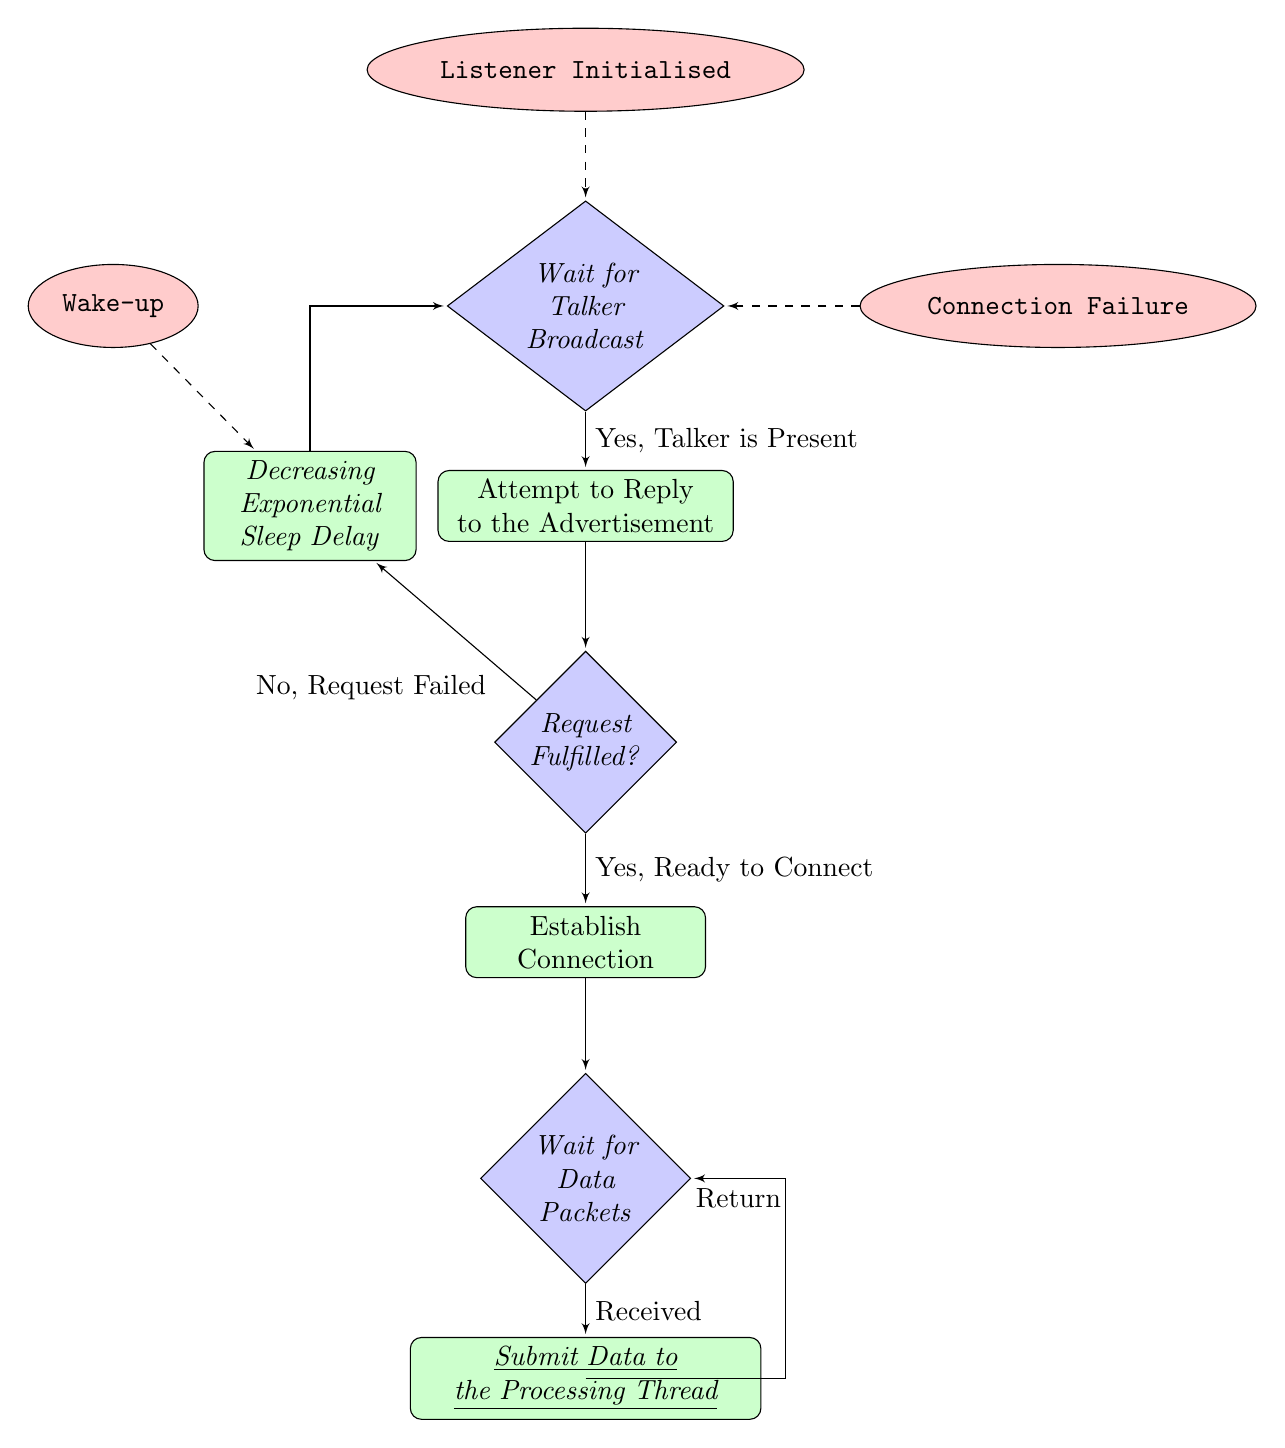
\begin{tikzpicture}[>=latex, shorten >=1pt, node distance=1in,
			on grid, auto, initial text=\fbox{\tt{Start}}]


\node [E]
(run)
	{\texttt{Listener Initialised}};

\node [C, below of =run, minimum width=10em]
(adv)
	{\emph{Wait for Talker Broadcast}};

\node [E, left of =adv, node distance =6cm]
(wup)
	{\texttt{Wake-up}};

\node [F, below of =adv, text width=10em]
(rep)
	{Attempt to Reply\\to the Advertisement};

\node [C, below of =rep]
(req)
	{\emph{Request Fulfilled?}};

\node [F, below of =req, text width=8em]
(con)
	{Establish Connection};

\node [C, below of =con]
(buf)
	{\emph{Wait for Data Packets}};

\node [F, below of =buf, text width=12em]
(use)
	{\emph{\underline{Submit Data to}\\\underline{the Processing Thread}}};

\node [E, right of =adv, node distance =6cm]
(int)
	{\texttt{Connection Failure}};

\node [F, left of =rep, node distance =3.5cm, text width=7em]
(del)
	{\emph{Decreasing\\Exponential\\Sleep Delay}};

\coordinate [right of =use] (ret);

\path[L, dashed] (run) -- (adv);

\path[L, dashed] (int) -- (adv);

\path[L, dashed] (wup) -- (del);

\path[L] (adv) -- node {Yes, Talker is Present} (rep);

\path[L] (rep) -- (req);

\path[L] (req) -- node [near start] {No, Request Failed} (del);

\path[L] (del) |- (adv);

\path[L] (req) -- node {Yes, Ready to Connect} (con);

\path[L] (con) -- (buf);

\path[L] (buf) -- node {Received} (use);

\path[L] (use) |- (ret) |- node [near end] {Return} (buf);

\end{tikzpicture}

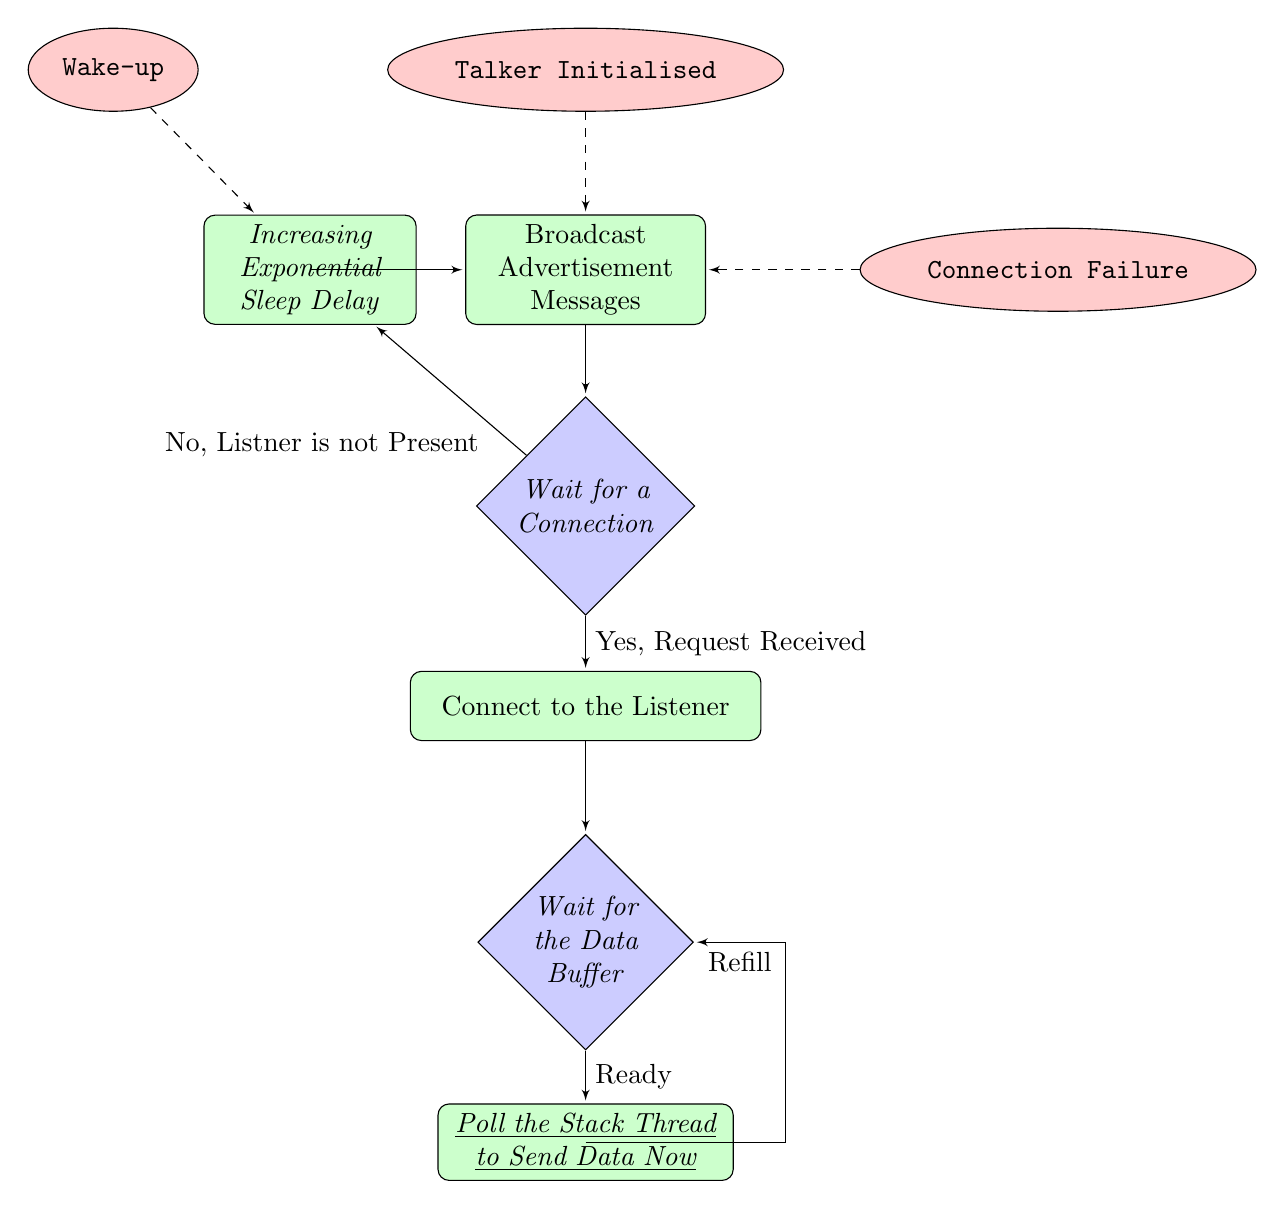
\begin{tikzpicture}[>=latex, shorten >=1pt, node distance=1in,
			on grid, auto, initial text=\fbox{\tt{Start}}]


\node [E]
(run)
	{\texttt{Talker Initialised}};

\node [E, left of =run, node distance =6cm]
(wup)
	{\texttt{Wake-up}};

\node [F, below of =run, text width=8em]
(adv)	
	{Broadcast Advertisement Messages};

\node [C, below of =adv, text width=6em]
(rep)
	{\emph{Wait for a Connection}};

\node [F, below of =rep, text width=12em]
(con)
	{Connect to the Listener};

\node [C, below of =con]
(buf)
	{\emph{Wait for the Data Buffer}};

\node [F, below of =buf, text width=10em]
(now)
	{\emph{\underline{Poll the Stack Thread}\\\underline{to Send Data Now}}};

\node [E, right of =adv, node distance =6cm]
(int)
	{\texttt{Connection Failure}};

\node [F, left of =adv, node distance =3.5cm, text width=7em]
(del)
	{\emph{Increasing\\Exponential\\Sleep Delay}};
\coordinate [right of =now] (ret);

\path[L, dashed] (run) -- (adv);

\path[L, dashed] (int) -- (adv);

\path[L, dashed] (wup) -- (del);

\path[L] (adv) -- (rep);

\path[L] (rep) -- node {Yes, Request Received} (con);

\path[L] (rep) -- node [near start] {No, Listner is not Present} (del);

\path[L] (del) |- (adv);

\path[L] (con) -- (buf);

\path[L] (buf) -- node {Ready} (now);

\path[L] (now) |- (ret) |- node [near end] {Refill} (buf);

\end{tikzpicture}


%%%%%%%%%%%%%%%%%%%%%%%%%%%%%%%%%%%%%%%%%%%%%%%%%%%%%%%%%%%%%%%%%%%%%%%%

\bibliographystyle{acm}

\bibliography{../main,../../contiki/dunkels}

\end{document}
